% -----
% COMP2550 proposal
% CHRISTOPHER CLAOUE-LONG
% -----
% -
% - DOCUMENT GEOMETRY SETUP
\documentclass[12pt,a4paper]{article}
\usepackage[margin=20mm]{geometry}
\usepackage{wrapfig}
\usepackage{lastpage} % to display the page number down the bottom
\makeatletter \renewcommand{\@oddfoot}{\hfil Page \thepage\ of \pageref{LastPage} \hfil} \makeatother % Page X of Y down the bottom
% -
% - FONT
\usepackage{amsmath,amsthm,amssymb,graphicx,epstopdf,datetime,multicol,verbatim,ulem,alltt,multirow}
\DeclareGraphicsRule{.tif}{png}{.png}{`convert #1 `dirname #1`/`basename #1 .tif`.png}
\usepackage[sc]{mathpazo} % Palatino maths fonts - acceptable fonts for typesetting, also sets these fonts for use in math mode
\linespread{1.05}
\usepackage[T1]{fontenc}
\usepackage[bitstream-charter]{mathdesign}
% -
% - MISC. PACKAGES
\usepackage[usenames,dvipsnames,svgnames,table]{xcolor}
\usepackage{hyperref}
\hypersetup{
colorlinks,
citecolor=black,		% - Citation colour
filecolor=black,		% - File colour
linkcolor=black,		% - Link colour
urlcolor=black		% - URL colour
}\urlstyle{same}
% -
% -
% - MISC. SYMBOLS AND COMMANDS
\newcommand{\HUGE}[1]{\textbf{\Huge #1}}
\newcommand{\ITALIC}[1]{\textit{#1}}
\newcommand{\BOLDL}[1]{\textbf{\large #1}}
\newcommand{\BOLD}{\textbf}
\newcommand{\Hrule}{\textcolor{blue}{\rule{\linewidth}{0.5mm}}} 
% Defines a new command for the horizontal lines, change thickness here
\newcommand{\htab}{\hspace*{0.63cm}}
% -
% -----
% BEGIN DOCUMENT
% -----
\begin{document}
% -----
% - Title
{\center{\Hrule\vspace{0.2em}
	%
	\HUGE{COMP2550/COMP3130 ANU\\Main Project Proposal}\\
	\BOLDL{
		Christopher Claou\'e-Long
		(\href{mailto:u5183532@anu.edu.au}
		{\ITALIC{\underline{\smash{u5183532@anu.edu.au}}}})\\
		Jimmy Lin 
		(\href{mailto:u5223173@anu.edu.au}
		{\ITALIC{\underline{\smash{u5223173@anu.edu.au}}}})\\
	}
	\BOLD{Last typeset: \currenttime, \today}
\\\Hrule}}
% -
% -
\begin{multicols}{2}
\section{Introduction}
[problem motivation, background, application...] \\
% introduce the related work in the area of saliency detection 
\htab There are a few existing works to achieve the functionality of detecting the salient objects. The mainstream appraoch in the last decade should be the (Itti,1998)'s algorithm (see ref.3). It outputs a feature map and then converts it to a rectangle by winner-take-all algorithm. But the precision of the detection is quite unsatisfying, even though it does hae a good recall. The second approach is the fuzzy-growing approach (see ref.4). But [badness of this approach...]. \\
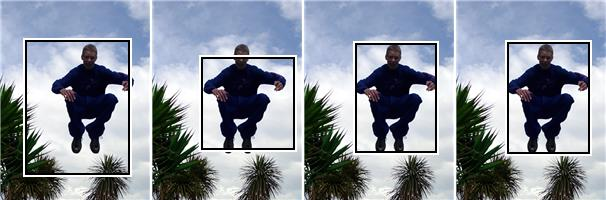
\includegraphics[width=3.2in,height=1in]{./pictures/0_imCanvs_Compare.jpg} \\
\figcaption{\footnotesize (a) FG(Ma,2003) (b) SM(Itti,1998) (c) CRFM(Liu,2007) (d) Ground truth} \\
% introduce the framework we referred to
\htab The research we referred to in this experimental project (see ref.2), which is based on conditional random field (CRF) model, has a large portion of perfect detection compared with ground truth data. At first stage, it extracts features in the local, regional and global level, corresponding to multiscale contrast, center-surround histogram and spatial color distribution respectively. And then after normalization and linear/non-linear combination, a master map or a salient map is computed to represent the saliency of each image pixel. Last, a few key locations on the saliency map are identified by winner-take-all or inhibition-of-return, or other non-linear operations.\\
% declare our work in this project and why we choose this as the topic of project
\htab Our implementation involves in utilizing the open-source library OpenCV and Darwin to achieve the framework of the CRF-based saliency detection. [why we choose this topic, (1) experience of implementing graphical model (2) it may help to scene understanding...]\\
\section{Formulation}
\subsection{CRF Model}
Model conditional distribution of objective variable 
    $$ P(A|I) = \frac{1}{Z} exp(-E(A|I)) $$
Energy function is formualted to be a set of static salient features and one pairwise feature as follows,
    $$ E(A|I) = \sum_{x} \sum_{k=1}^{K} \lambda_{k} F_{k}(a_{x},I)  
        + \sum_{x,x'} S(a_{x},a_{x'},I)  $$ \vspace{-0.4cm}
\begin{center} \footnotesize $\lambda_{k}$: weight of $k$th feature, $x,x'$: two adjacent pixels. \end{center} 

\subsection{Feature Extraction}
\textbf{Multiscale Contrast}. This static feature captures the high contrast in the boundary of objects . \\[0.1cm]
\textbf{Center-Surround Histogram}. This static feature captures  \\[0.1cm]
\textbf{Spatial Color distribution}. This static feature penalizes the pixels with widely distributed color. \\[0.1cm]
\textbf{Pairwise Feature}. This feature exploits the spatial relationship between two adjacent pixels and can be viewed as one capturing the spatial continuity of saliency, that is, adjacent pixels that are prone to be assigned with different labels. 
\subsection{Possible Improvements}
[more features that better capture the saliency...]

\section{Project Timeline}
Apr. 1st $\Rightarrow$ Apr. 18th \\
\textbf{Project Proposal}. Read papers to find project of our interest, determine the topic of our second project and collect relevant data sets for training. \\[0.2cm]
Apr. 19th $\Rightarrow$ Apr. 28th  \\
 \textbf{Framework Construction}. Familiarize ourself with the related packages in Darwin and OpenCV, set up the interface to accept training data and the framework of CRF model for learning and inference.   \\[0.2cm]
Apr. 29th $\Rightarrow$ May. 12th \\
 \textbf{Intensive Coding}. Write codes to implement extraction of various features, and design the algorithm to output a rectangle labeling saliency. \\[0.2cm]
May. 12th $\Rightarrow$ May. 19th \\
\textbf{Testing, Enhancement}. Test the framework we would have constructed. Search and implement possible improvements. \\[0.2cm] 
May. 20th $\Rightarrow$ May. 30th \\
\textbf{Project Summarization}. Write report to summarize our project and make presentation. \\
% References
\begin{thebibliography}{8}
    \footnotesize
    \bibitem 1 Gould, Stephen. "DARWIN: A Framework for Machine Learning and Computer Vision Research and Development." \textit{Journal of Machine Learning Research 13 (2012): 3533-3537}. 
    \bibitem 2 Liu, Tie, et al. "Learning to detect a salient object." \textit{Pattern Analysis and Machine Intelligence, IEEE Transactions on 33.2 (2011): 353-367}. 
    \bibitem 3 Itti, Laurent, Christof Koch, and Ernst Niebur. "A model of saliency-based visual attention for rapid scene analysis."\textit{ Pattern Analysis and Machine Intelligence, IEEE Transactions on 20.11 (1998): 1254-1259}.
    \bibitem 4 Ma, Yu-Fei, and Hong-Jiang Zhang. "Contrast-based image attention analysis by using fuzzy growing."\textit{ Proceedings of the eleventh ACM international conference on Multimedia. ACM, 2003}. 
\end{thebibliography}

\end{multicols}

\vfill\Hrule
\end{document}
% -----
% END OF LINE
% -----
